% !TEX encoding = UTF-8
% !TEX TS-program = pdflatex
% !TEX root = ../tesi.tex

%**************************************************************
\chapter{Analisi del problema e studio delle tecnologie}
\label{cap:progetto-stage}
%**************************************************************

\section{Specifiche tecniche del problema}

Nel primo periodo di stage, il tempo è stato dedicato allo studio delle componenti del problema da affrontare, ricavando un quadro generale del
funzionamento logico della pianificazione della produzione. 
Perché un prodotto venga pianificato, è necessario che ci sia almeno una linea in grado di produrlo, una volta definita la linea si deve scegliere una sequenza in 
cui produrre l'articolo. Una sequenza definisce giorno, data di inizio e di fine e può comprendere un insieme di vincoli da soddisfare
(quali lavaggi oppure ordinaria manutenzione), l'articolo verrà quindi inserito all'interno della sequenza con il relativo tempo di produzione.
Ogni linea ha solitamente più sequenze, nelle quali è possibile collocare l'articolo. Ogni sequenza può avere dei vincoli di dipendenza con altre sequenze.


\subsection{Elementi del sistema da ottimizzare}
Segue la descrizione della struttura, ad alto livello, riguardante le principali meccaniche che definiscono il problema di ottimizzazione e da considerare nello sviluppo dell'applicativo.

\subsubsection{Linee}
Indica l'insieme delle linee sulle quali è consentita la produzione degli ordini, ogni linea ha relativo costo orario e definisce l'insieme degli articoli che può produrre con annessa velocità di produzione.
Ogni linea è così definita:
\begin{itemize}
	\item \textbf{Codice Linea}: serve ad indicare su quale linea si vuole produrre l'articolo;
	\item \textbf{Info Articolo}: lista che indica quali articoli la linea può produrre con relativo tempo di produzione;
	\item \textbf{Info Vincolo}: lista che indica i vincoli presenti sulla linea, possono essere obbligatori o opzionali;
	
	\item \textbf{Sequenze Linea}: lista che indica quali sono le sequenze di produzione della linea;
	
	\item \textbf{Pianificazione}: lista che indica quali articoli e quali vincoli sono stati pianificati nella linea corrente;
	
	
	\item \textbf{Errori}: indica quali errori si sono presentati durante la pianificazione;
	
	\item \textbf{Calendario}: indica quali sono i giorni lavorativi con le eventuali pause.
	
\end{itemize}

\subsubsection{Sequenze}
Indica l'insieme delle sequenze di produzione presenti su ogni linea, nelle quali vengono inseriti gli ordini che sono stati pianificati.
Ogni sequenza è così definita:
\begin{itemize}
	\item \textbf{Codice Sequenza}: serve ad indicare su quale sequenza si vuole inserire l'articolo;
	\item \textbf{Giorno}: indica il giorno nel quale si vuole inserire l'articolo;
	\item \textbf{Ora inizio/Ora fine}: indica gli orari di inizio e fine della sequenza corrente;
	
	\item \textbf{Elementi}: lista che indica gli articoli e i vincoli appartenenti alla sequenza corrente.
	
\end{itemize}

\subsubsection{Ordine}
Indica come si presenta un ordine da produrre.
Ogni ordine è così definito:
\begin{itemize}
	\item \textbf{Codice Articolo}: indica il codice dell'articolo;
	\item \textbf{Tipo Articolo}: indica il tipo dell'articolo, può essere un prodotto finito, semilavorato o materia prima;
	\item \textbf{Codice Linea}: indica il livello più generale della gerarchia di classificazione di un prodotto;
	\item \textbf{Codice Settore}: indica il terzo livello di gerarchia di classificazione;
	\item \textbf{Codice Famiglia}: indica il secondo livello di gerarchia, definisce la famiglia del prodotto;
	\item \textbf{Codice SottoFamiglia}: indica il livello più caratterizzante della classificazione di un prodotto;
	
	\item \textbf{Quantità}: indica la quantità richiesta da produrre;
	
	\item \textbf{Data Spedizione}: indica la data di spedizione dell'articolo;
	
	\item \textbf{Ora spedizione}: indica l'ora di spedizione dell'articolo;
	
	\item \textbf{Data Consegna}: indica la data di consegna presso la sede del cliente;
	 
	\item \textbf{Linea preferenziale}: indica la linea preferenziale di produzione dell'articolo;
	
	\item \textbf{Anno Ordine}: indica l'anno dell'ordine in questione; 

    \item \textbf{Materie Prime}: lista che indica l'insieme delle materie prime richieste per la produzione dell'ordine;
  
   \item \textbf{Semilavorati}: lista che indica l'insieme dei semilavorati richiesti per la produzione dell'ordine;
   
   \item \textbf{Riferimento Ordine}: lista che indica l'insieme degli ordini ai quali l'ordine corrente fa riferimento per la produzione di semilavorati;
   
\end{itemize}

\subsection{Vincoli del problema}
Di seguito sono presentate i vincoli e le specifiche che un metodo di ottimizzazione per il sistema in esame deve considerare per ottenere una corretta pianificazione della produzione.

\subsubsection{Vincoli temporali}
I vincoli riguardanti i tempi di produzione sono legati a:
\begin{itemize}
	\item \textbf{Data Spedizione}: devono essere rispettate le date di spedizione e di consegna degli articoli da pianificare;
	\item \textbf{Tempo minimo alla consegna}: devono essere rispettate le date di inizio produzione nel caso di ordini con scadenza a breve termine;
	
	\item \textbf{Semilavorati}: i semilavorati di un ordine devono essere pianificati prima dell'ordine stesso;
	
	\item \textbf{Ordini Fornitori}: vanno considerate le date di arrivo delle materie prime da parte dei fornitori in modo da non scartare la produzione di ordini che sarebbero producibili;
	
	\item \textbf{Giorni Lavorativi}: devono essere rispettati i giorni lavorativi senza pianificare ordini al di fuori di essi;
	\item \textbf{Orario Lavorativo}: devono essere rispettati gli orari lavorativi senza eccedere dal monte ore impostato dall'azienda che esegue la pianificazione;
	\item \textbf{Sovrapposizione Sequenze}: ogni linea può produrre una singola sequenza per volta;	
	\item \textbf{Sovrapposizione Articoli}: ogni sequenza può contenere un solo articolo senza sovrapporne degli altri nello stesso lasso di tempo.
\end{itemize}

\subsubsection{Vincoli di produzione}
I vincoli da rispettare sono:
\begin{itemize}
	
	\item \textbf{Materie prime}: non è possibile produrre un ordine se non sono presenti sufficienti materie prime;
	
	\item \textbf{Vincoli Obbligatori}: devono essere pianificati tutti i vincoli obbligatori di ogni sequenza;
	\item \textbf{Vincoli Condizionati}: devono essere pianificati tutti i vincoli condizionati di ogni sequenza in base alle condizioni imposte;
\item \textbf{Vincoli Opzionali}: devono essere pianificati i vincoli opzionali solo in caso ci sia una finestra temporale sufficiente altrimenti si lascia spazio alla produzione di articoli;
	\item \textbf{Vincoli Articolo}: devono essere rispettati i vincoli di produzione di ogni articolo, quali linea preferenziale o linea con maggiore velocità di produzione.
\end{itemize}

\subsubsection{Scelte implementative}
Dopo una discussione col tutor interno abbiamo scartato l'ultimo vincolo facoltativo FA2, presente nel piano di lavoro, il quale riguardava la ripianificazione
degli articoli in caso di guasti o necessità aziendali, optando per una semplice nuova esecuzione dell'applicativo con i nuovi dati interessati. 



\section{Analisi dei requisiti}

Uno dei requisiti vincolava la modifica a livello grafico dell'applicativo, in quanto la clientela era abituata alla versione corrente e non sempre
è immediato adattarsi a cambiamenti di questo tipo.\\ 
Si è quindi fatto affidamento all'analisi dei requisiti stilata dallo stagista precedente \hyperref[analisi-requisiti]{[3]}.
Sono stati aggiunti due casi particolari che verranno evidenziati di seguito.

%************************************************************

\subsection{Casi d'uso}

Per rappresentare l'insieme delle azioni comuni ad un singolo utente sono stati utilizzati i casi d'uso.
Per descrivere i vari scenari ho mantenuto la precedente scaletta di informazioni così da dare una continuità al documento esistente. 
Ciascun caso d'uso sarà quindi rappresentato come descritto di seguito:
\begin{itemize}
    \item \textbf{Identificatore} univo nel formato UC-[Codice];
    \item \textbf{Titolo} del caso d'uso;
    \item \textbf{Descrizione} generale del caso d'uso;
    \item \textbf{Attori} coinvolti: primari e secondari;
    \item \textbf{Precondizione} del caso d'uso;
    \item \textbf{Scenario principale} che il caso d'uso vuole modellare, identificando ogni azione che ne fa parte;
    \item \textbf{Postcondizione} del caso d'uso;
    \item \textbf{Estensioni} dello scenario principale, evidenziata da una lettera maiuscola e inserita in un elenco.
\end{itemize}

Di seguito vengono rappresentate le modifiche apportate al documento esistente\hyperref[analisi-requisiti]{[3]}.
Si fa riferimento allo standard UML 2.0 \hyperref[uml]{[4]} per la rappresentazione dei casi d'uso.

\subsection*{UC-3 Pianificazione della produzione}

\begin{figure}[H]
	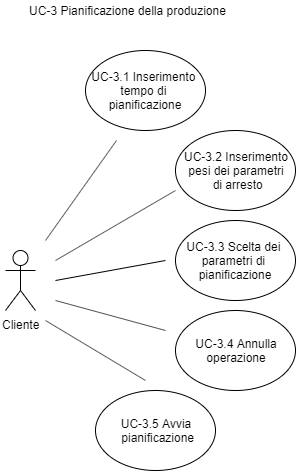
\includegraphics[width=8cm]{immagini/UC1.png}
	\centering
	\caption{Use Case - UC-3}
\end{figure}

\textbf{Attori}: Cliente. \newline
\textbf{Descrizione}: Il cliente esegue la pianificazione degli ordini selezionati.\newline
\textbf{Precondizione}: Il cliente ha selezionato gli ordini che intende pianificare e i giorni in cui vuole farlo.\newline
\textbf{Scenario principale}: \begin{itemize}
    \item Il cliente seleziona che ordini vuole pianificare;
    \item Il cliente preme il pulsante "Pianifica";
    \item Il cliente modifica i parametri della pianificazione come previsto dagli UC-3.1, UC-3.2, UC-3.3;
    \item Il cliente preme il pulsante "Avvia pianificazione".
\end{itemize}

\textbf{Postcondizione}: Nella finestra principale viene visualizzato il risultato della pianificazione.


\subsection*{UC-3.3 Scelta dei parametri di pianificazione}

\begin{figure}[H]
	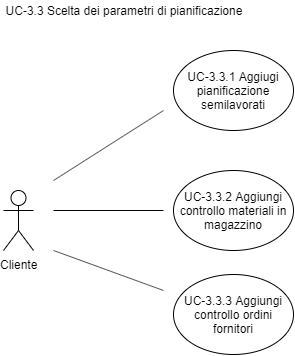
\includegraphics[width=8cm]{immagini/UC2.png}
	\centering
	\caption{Use Case - UC-3.3}
\end{figure}

\textbf{Attori}: Cliente. \newline
\textbf{Descrizione}: Il cliente seglie i parametri da considerare nella pianificazione.\newline
\textbf{Precondizione}: Il cliente ha selezionato il pulsante "Metodo di pianificazione".\newline
\textbf{Scenario principale}: \begin{itemize}
    \item Il cliente seleziona come effettuare le pianificazione;
    \item Il cliente può selezionare le varie aggiunte descritte dagli UC-3.3.1, UC-3.3.2, UC3.3.3;
    \item Il cliente preme il pulsante "Conferma".
\end{itemize}
\textbf{Postcondizione}: Si verrà ricondotti allo use case UC-3.3.
\newpage
\section{Tracciamento dei requisiti}

Ogni requisito è composto dalla seguente struttura:
\begin{itemize}
	\item \textbf{codice identificativo}: ogni codice identificativo è univoco e conforme alla seguente codifica:\\
	\centerline{\textbf{RE[Importanza][Tipologia][Codice]}} \\ \\
	Il significato delle cui voci è:
	\begin{itemize}
		\item \textbf{Tipologia}: ogni requisito può assumere uno dei seguenti valori:
		\begin{itemize}
			\item \textit{F}: funzionale;
			\item \textit{P}: prestazionale;
			\item \textit{Q}: qualitativo;
			\item \textit{V}: vincolo.
		\end{itemize}
		\item \textbf{Importanza}: ogni requisito può assumere uno dei seguenti valori:
		\begin{itemize}
			\item \textit{O}: requisito obbligatorio: irrinunciabili per qualcuno degli stakeholder;
			\item \textit{D}: requisito desiderabile: non strettamente necessari ma  a valore aggiunto riconoscibile;
			\item \textit{F}: requisito facoltativo: relativamente utili oppure contrattabili più avanti nel progetto.	
		\end{itemize}
		\item \textbf{Codice}: è un identificatore univoco del requisito segue un ordine incrementale.
	\end{itemize}
	\item \textbf{classificazione}: viene riportata l'importanza del requisito. Sebbene questa sia un'informazione ridondante ne facilita la lettura;
	\item \textbf{descrizione}: descrizione breve ma completa del requisito, meno ambigua possibile.
\end{itemize}
\renewcommand{\arraystretch}{1.5}



\subsection{Requisiti funzionali}

L'insieme delle funzionalità che il sistema deve fornire vengono definite nella \hyperref[3.1]{Tabella 3.1}.

\renewcommand{\arraystretch}{1.5}
\rowcolors{2}{dispari}{pari}
\arrayrulecolor{white}

\begin{longtable}{ >{\centering}p{0.15\textwidth} >{\centering}p{0.20\textwidth}
		>{\raggedright}p{0.35\textwidth} >{\centering}p{0.14\textwidth}}
	\caption{Tabella dei requisiti funzionali}
	\label{3.1}
	\\
	\rowcolorhead 
	\textbf{\color{white}Requisito} 
	& \textbf{\color{white}Classificazione} 
	& \centering\textbf{\color{white}Descrizione}
	 
	\endfirsthead
	\rowcolor{white}\caption[]{(continua)}\\
	\rowcolorhead 
	\textbf{\color{white}Requisito} 
	& \textbf{\color{white}Classificazione} 
	& \centering\textbf{\color{white}Descrizione}
	
	\endhead	
	
	REFO1	&	Obbligatorio	&	Il sistema permette l’inserimento di un nuovo vincolo di linea	 \tabularnewline
	REFO2	&	Obbligatorio	&	Il sistema permette la modifica dei dati di un vincolo di linea esistente	\tabularnewline
	REFO3	&	Obbligatorio	&	Il sistema permette l’eliminazione di un vincolo di linea 	\tabularnewline
	REFO4	&	Obbligatorio	&	L’interfaccia permette l’eliminazione di una linea 	\tabularnewline
	REFO5	&	Obbligatorio	&	 Il sistema permette l’aggiunta di una nuova sequenza	\tabularnewline
	REFO6	&	Obbligatorio	&	 Il sistema permette la modifica dei dati di una sequenza esistente	\tabularnewline
	REFO7	&	Obbligatorio	&	 Il sistema permette l’eliminazione di un articolo di sequenza esistente	\tabularnewline
	REFO8	&	Obbligatorio	&	 Il sistema permette l’eliminazione di un vincolo di sequenza esistente	\tabularnewline
	REFO9	&	Obbligatorio	&	 Il sistema permette l’eliminazione di una sequenza	\tabularnewline
	REFO10	&	Obbligatorio	&	 Il sistema permette all’utente di scegliere un tempo massimo di esecuzione dell’algoritmo	\tabularnewline
	REFO11	&	Obbligatorio	&	 Il sistema permette all’utente di assegnare un peso all’importanza di parametri di produzione quali:pezzi prodotti e occupazione delle linee	\tabularnewline
	REFD1	&	Desiderabile	&	 Il sistema permette all’utente di scegliere se ricalcolare la pianificazione già esistente	\tabularnewline
	REO12	&	Obbligatorio	&	 Il sistema permette di pianificare automaticamente la produzione dato un insieme di ordini e un intervallo di tempo	\tabularnewline
	REFO1	&	Obbligatorio	&	 Il sistema permette di scegliere i relativi criteri di pianificazione	\tabularnewline
\end{longtable}

\newpage
\subsection{Requisiti qualitativi}

Vengono illustrati nella \hyperref[3.2]{Tabella 3.2} i requisiti che incrementano la qualità generale del sistema.

\rowcolors{2}{pari}{dispari}

\begin{longtable}{ >{\centering}p{0.15\textwidth} >{\centering}p{0.20\textwidth}
		>{\raggedright}p{0.35\textwidth} >{\centering}p{0.14\textwidth}}
	\caption{Tabella dei requisiti qualitativi}
	\label{3.2}
	\\
	\rowcolorhead 
	\textbf{\color{white}Requisito} 
	& \textbf{\color{white}Classificazione} 
	& \centering\textbf{\color{white}Descrizione}
	 
	\endfirsthead
	\rowcolor{white}\caption[]{(continua)}\\
	\rowcolorhead 
	\textbf{\color{white}Requisito} 
	& \textbf{\color{white}Classificazione} 
	& \centering\textbf{\color{white}Descrizione}
	
	\endhead	
	
	REQD1	&	Desiderabile	&	Il programma genera un file di \hyperref[Log]{Log\glo} di supporto al \hyperref[Debug]{Debug\glo}	 \tabularnewline
	REQO1	&	Obbligatorio	&	Ogni scelta non banale effettuata è adeguatamente commentata nel codice	\tabularnewline
	REQF1	&	Facoltativo		&	Fornire un manuale utente	\tabularnewline
	REQF2	&	Facoltativo		&	Fornire un manuale sviluppatore	\tabularnewline

\end{longtable}

\subsection{Requisiti prestazionali}

La \hyperref[3.3]{Tabella 3.3} definisce i requisiti riguardanti le prestazioni attese dal software.

\rowcolors{2}{pari}{dispari}

\begin{longtable}{ >{\centering}p{0.15\textwidth} >{\centering}p{0.20\textwidth}
		>{\raggedright}p{0.35\textwidth} >{\centering}p{0.14\textwidth}}
	\caption{Tabella dei requisiti prestazionali}
	\label{3.3}
	\\
	\rowcolorhead 
	\textbf{\color{white}Requisito} 
	& \textbf{\color{white}Classificazione} 
	& \centering\textbf{\color{white}Descrizione}
	 
	\endfirsthead
	\rowcolor{white}\caption[]{(continua)}\\
	\rowcolorhead 
	\textbf{\color{white}Requisito} 
	& \textbf{\color{white}Classificazione} 
	& \centering\textbf{\color{white}Descrizione}
	
	\endhead	
	
	REPD1	&	Desiderabile	&	L'applicativo deve fornire una soluzione entro il tempo stabilito dall'utente	 \tabularnewline
	REPD2	&	Desiderabile	&	L'applicativo deve fornire la soluzione nel modo più rapido possibile senza valutare ulteriori combinazioni se è stato
	raggiunto un determinato punteggio stabilito per la soluzione stessa \tabularnewline
	REPD3	&	Desiderabile	&	La fase di lettura dei dati deve essere eseguita in tempi inferiori ai 30 minuti \tabularnewline

\end{longtable}
\newpage
\subsection{Requisiti vincolo}

La \hyperref[3.4]{Tabella 3.4} definisce i requisiti vincolanti per l'integrazione di nuove componenti nel sistema preesistente.

\rowcolors{2}{pari}{dispari}

\begin{longtable}{ >{\centering}p{0.15\textwidth} >{\centering}p{0.20\textwidth}
		>{\raggedright}p{0.35\textwidth} >{\centering}p{0.14\textwidth}}
	\caption{Tabella dei requisiti prestazionali}
	\label{3.4}
	\\
	\rowcolorhead 
	\textbf{\color{white}Requisito} 
	& \textbf{\color{white}Classificazione} 
	& \centering\textbf{\color{white}Descrizione}
	 
	\endfirsthead
	\rowcolor{white}\caption[]{(continua)}\\
	\rowcolorhead 
	\textbf{\color{white}Requisito} 
	& \textbf{\color{white}Classificazione} 
	& \centering\textbf{\color{white}Descrizione}
	
	\endhead	
	
	REVO1	&	Desiderabile	&    Rendere compatibile il programma con l’attualemodulo di pianificazione della produzione	 \tabularnewline
	REVO2	&	Desiderabile	&    Ottimizzare la pianificazione tenendo conto delle materie prime e dei semilavorati	 \tabularnewline
	REVO3	&	Desiderabile	&    Ottimizzare la pianificazione tenendo conto degli ordini dei fornitori inseriti a sistema	 \tabularnewline
	REVO4	&	Desiderabile	&    Ottimizzare la pianificazione rendendo possibile la pianificazione dei semilavorati	 \tabularnewline
	REVO5	&	Desiderabile	&    Il programma è sviluppato tramite il linguaggio diprogrammazione Vb.NET v.4.7.0	 \tabularnewline
	REVO6	&	Desiderabile	&    \hyperref[IDE]{L’IDE\glo} (Integrated development environment) utilizzato è Microsoft Visual Studio v.10.0.4	 \tabularnewline
	REVO7	&	Desiderabile	&    Le componenti grafiche sono basate sulle DevEx-press	 \tabularnewline
	REVO8	&	Desiderabile	&    I dati vengono salvati su un database Informix	 \tabularnewline
	REVO9	&	Desiderabile	&    I dati in input sono scritti su un file JSON	 \tabularnewline
	REVO10	&	Desiderabile	&    I dati in output sono scritti su un file JSON	 \tabularnewline

\end{longtable}

\newpage
\subsection{Riepilogo dei requisiti}

La \hyperref[3.5]{Tabella 3.5} riassume l'insieme dei requisiti che il sistema deve soddisfare.

\rowcolors{2}{pari}{dispari}

\begin{longtable}{ >{\centering}p{0.15\textwidth} >{\centering}p{0.20\textwidth}
		>{\centering}p{0.35\textwidth} >{\centering}p{0.14\textwidth}}
	\caption{Tabella del riepilogo dei requisiti}
	\label{3.5}
	\\
	\rowcolorhead 
	\textbf{\color{white}Tipo} 
	& \textbf{\color{white}Obbligatori} 
	& \centering\textbf{\color{white}Desiderabili}
	& \centering\textbf{\color{white}Facoltativi}
	
	\endhead	
	
	Funzionali	&	13	&  1  &	0 \tabularnewline
	Qualitativi	&	1	&  1  &	 2 \tabularnewline
	Prestazionali	&	0	&   3 & 0	 \tabularnewline
	Di vincolo	&	10	& 0   &	0 \tabularnewline
	Totali	&	24	&   5 &	2 \tabularnewline

\end{longtable}
\newpage
\section{Tecnologie e strumenti}

Di seguito sono riportate tutte le tecnologie utilizzate durante lo sviluppo del progetto.
Tali scelte sono state imposte da Ergon Informatica in quanto sono gli strumenti che vengono utilizzati dall'azienda per lo sviluppo dei progetti interni.\\
La scelta è inoltre guidata dal fatto che, per mantenere l'integrazione con le parti già esistenti dell'applicativo e il suo funzionamento tramite il software Ergdis, 
non è stato possibile spostarsi su nuove tecnologie, magari anche solo a qualche versione successiva di esse.\\
Ergon Informatica si appoggia a questi strumenti in quanto sono forniti di un ottima documentazione di supporto, hanno un alto tasso di scalabilità 
e forniscono un supporto in tempo reale alla codifica.\\ \\

\textbf{Vb.NET}

Vb.NET, il cui logo è mostrato in \hyperref[net]{Figura 3.3}, è linguaggio di programmazione che deriva da Visual Basic 6,
 è sviluppato da Microsoft e, al contrario dei precedenti, supporta il paradigma di programmazione
orientata agli oggetti \hyperref[vbnet]{[5]}.

\begin{figure}[H]
	
\includegraphics[width=5cm]{immagini/vb.png}
	\centering
	\caption{Logo Vb.NET\hyperref[vb-logo]{[6]}}
	\label{net}
\end{figure}

Vb.NET consente lo sviluppo di applicazioni Windows, Web e per dispositivi mobili. \\
Come avviene con tutti i linguaggi basati su Microsoft .NET Framework,
i programmi scritti in Vb.NET usufruiscono delle funzionalità di sicurezza e interoperabilità dei linguaggi.\\
Nel progetto viene utilizzato questo linguaggio per poter usufruire delle classi, le quali riducono significativamente le duplicazioni di codice e rendono l'intero sorgente 
chiuso alle modifiche e aperto agli ampliamenti. \\Viene inoltre utilizzato in quanto è il linguaggio attualmente adottato dall'azienda per lo sviluppo e si presta bene
al tipo di lavorazioni necessarie a portare a compimento lo sviluppo dell'applicativo.

\newpage
\textbf{Visual Studio 2010}\\
Visual Studio 2010, il cui logo è mostrato in \hyperref[vs-2010]{Figura 3.4}, è un ambiente di sviluppo integrato sviluppato da Microsoft \hyperref[vs]{[7]}. 
\begin{figure}[H]
	
\includegraphics[width=9cm]{immagini/microsoft-visual-studio-2010-logo.png}
	\centering
	\caption{Logo Visuali Studio 2010 \hyperref[vs-logo]{[8]}}
	\label{vs-2010}
\end{figure}


La prima versione risale al 1997 con lo scopo di fornire
un ambiente di sviluppo grafico ed integrato che aiutasse lo sviluppatore a gestire i progetti in maniera semplice, ma efficace, aumentandone quindi la produttività.\\
Microsoft ha incluso il supporto a differenti linguaggi di programmazione.\\
In Ergon Informatica è il principale ambiente di sviluppo sia per applicazioni desktop che mobile, di conseguenza è stato utilizzato anche durante lo sviluppo del progetto.\\

\textbf{DevExpress}\\

\textit{Developer Express Inc.}, il cui logo è mostrato in \hyperref[dev-exp]{Figura 3.5}, è una società di sviluppo software fondata nel 1998, inizialmente fornisce un insieme di controlli 
\hyperref[UI]{UI\glo} poi sviluppa diverse estensioni per le librerie grafiche \hyperref[devexpress]{[9]}.

\begin{figure}[H]
	\includegraphics[width=8cm]{immagini/devexpress.png}
	\centering
	\caption{Logo DevExpress \hyperref[devlogo]{[10]}}
	\label{dev-exp}
\end{figure}

In particolare nel progetto ci si è appoggiati a questa tecnologia per velocizzare la creazione dell'interfaccia grafica sulla quale si basa il modo di rappresentare la soluzione
che viene fornita, permettendo una chiara visualizzazione tabellare grazie ad una delle tante \hyperref[Estensioni]{estensioni\glo} utilizzabili. 

\newpage

\textbf{JSON}

Acronimo di \textit{JavaScript Object Notation}, il cui logo è mostrato in \hyperref[js]{Figura 3.6}, è un formato adatto
all'interscambio di dati fra applicazioni \hyperref[Client/Server]{client/server\glo} \hyperref[json]{[11]}.

\begin{figure}[H]
	
\includegraphics[width=3cm]{immagini/json.png}
	\centering
	\caption{Logo JSON \hyperref[jlogo]{[12]}}
	\label{js}
\end{figure}

Serve, in particolare, a fornire una struttura a dati interessati rendendoli interscambiabili tra diverse applicazioni senza che si renda necessaria la codifica e decodifica di quest'ultimi.
Nel nostro caso si rende utile quando è necessario delegare l'esecuzione di operazioni sui dati prelavati da un terminale con accesso al database verso un terminale esterno.
I dati raccolti dal database venivano trasferiti in un file JSON, il quale veniva inviato al successivo passo di esecuzione dell'algoritmo, al termine di ciò veniva restituita
la soluzione sempre in formato JSON a chi ne aveva fatto richiesta e di conseguenza visualizzata.\\

\textbf{Informix}

Informix, il cui logo è mostrato in \hyperref[ibm]{Figura 3.7}, fa parte della divisione \hyperref[DBMS]{DBMS\glo} (Database Management System) di IBM, è un sistema software progettato per consentire la creazione,
la manipolazione e l'interrogazione efficiente di database \hyperref[informix]{[13]}.

\begin{figure}[H]
	\includegraphics[width=7cm]{immagini/Informix.png}
	\centering
	\caption{Logo Informix \hyperref[ilogo]{[14]}}
	\label{ibm}
\end{figure}


L'Informix server supporta il modello relazionale ad oggetti che permette ad IBM di offrire estensioni che supportano i tipi di dati che non sono una parte dello standard SQL.
Le estensioni più usate sono quelle riguardanti le serie temporali e spaziale che forniscono entrambe supporto al tipo di dato ed estensioni linguistiche che permettono 
interrogazioni per un dominio specifico ad alte prestazioni e archiviazione efficiente per set di dati basati su serie temporali e dati spaziali.
È il servizio database sul quale fa affidamento l'azienda, essendo IBM uno dei partner principali di Ergon Informatica.